\documentclass[11pt]{article}
\usepackage{amsthm}
\usepackage{amsmath}
\usepackage{amssymb}
\usepackage[spanish,es-tabla]{babel}
\usepackage[style=numeric,sorting=none]{biblatex}
\usepackage{bm}
\usepackage{booktabs}
\usepackage{enumitem}
\usepackage{fancyhdr}
\usepackage{float}
\usepackage[utf8]{inputenc}
\usepackage{listingsutf8}
\usepackage[top=2.5cm,bottom=2.5cm,left=2.5cm,right=2.5cm]{geometry}
\usepackage{graphicx}
\usepackage{longtable}
\usepackage{multicol}
%\usepackage{subcaption}
\usepackage{subfig}
\usepackage{verbatim}
\usepackage{xcolor}
\usepackage{xstring}

\definecolor{codegreen}{rgb}{0,0.6,0}
\definecolor{codegray}{rgb}{0.5,0.5,0.5}
\definecolor{codepurple}{rgb}{0.58,0,0.82}
\definecolor{backcolour}{rgb}{0.99,0.995,0.99}

\lstdefinestyle{mystyle}{
    backgroundcolor=\color{backcolour},   
    commentstyle=\color{codegreen},
    keywordstyle=\color{magenta},
    numberstyle=\tiny\color{codegray},
    stringstyle=\color{codepurple},
    basicstyle=\ttfamily\small,
    breakatwhitespace=false,         
    breaklines=true,                 
    captionpos=b,                    
    keepspaces=true,                 
    numbers=left,                    
    numbersep=5pt,                  
    showspaces=false,                
    showstringspaces=false,
    showtabs=false,                  
    tabsize=2
}
%\label{ tab: \StrBefore{#1}{.} } 

\newcommand{\figura}[3]{\begin{figure}[H] \centering \includegraphics[#3]{#1} \caption{#2} \label{#1}  \end{figure}}
\newcommand{\tablasimple}[2]{\begin{table}[H] \centering \input{#1} \caption{#2} \label{#1} \end{table}}
\newcommand{\tablalarga}[2]{ \begin{center} \input{#1} \begin{table}[H] \caption{#2} \label{#1} \end{table} \end{center}}

\lstset{style=mystyle}
\decimalpoint
% Adding references
\addbibresource{../../referencias.bib}
% Auxiliar commands
\newcommand{\work}{Tarea-Examen 5-6: Selección de modelos y regularización}
% Changes space between lines of equations
\setlength{\jot}{10pt}
% Changes space between text and equations
\setlength{\abovedisplayskip}{100pt}
\setlength{\belowdisplayskip}{100pt}
\setlength{\abovedisplayshortskip}{100pt}
\setlength{\belowdisplayshortskip}{100pt}
% Theorem environment in case I need it
\newtheorem{theorem}{Teorema}
% make header
\pagestyle{fancy}
\fancyhf{}
\vspace{1cm}
\rhead{}
\lhead{\work}
\cfoot{\thepage}
%  Text info
\title{\textbf{\work}}
\author{Curso Avanzado de Estadística. Profa. Guillermina Eslava Gómez.\\ \\ Aldo Sayeg Pasos Trejo. César Cossio Guerrero. \\ \\ Posgrado en Ciencias Matemáticas. Universidad Nacional Autónoma de México. }
\date{\today}
\begin{document}
\maketitle
\section{Problema 1}
Para el conjunto de datos ``Boston'', que consta de 13 variables numéricas y un variable categórica, buscamos predecir la variable \texttt{crim} como función de las otras 13 variables y sus interacciones a pares, lo que nos da $13 + \binom{13}{2} + 1 = 91$ variables predictoras.
\\
\\Notemos que las escalas de los datos son muy distintas entre cada variable, por lo se estandarizaron todas las variables numéricas para que tengan promedio $0$ y error estándar $1$. La variable categórica, al ser una indicadora, se dejó igual. 
\\
\\Posteriormente, se buscó cual era el valor de $l$ tal que al aplicar una transformación Box-Cox a \texttt{crim} se maximizaba la probabilidad de tener un comportamiento normal. Se encontro que $l = -0.11$ y se realizó la transformación a la variable respuesta.
\\
Probaremos siete modelos: tres sin regularizar, tres regularizados y uno utilizando un random forest regressor.
\subsection{Modelo normal}
Antes de escoger los modelos, realizamos un ajuste con un modelo normal de mínimos cuadrados que usa todas las variables. La tabla \ref{base.tex} muestra as estadísticas de dicho modelo.
\tablasimple{base.tex}{Estadísticas del modelo base. Los errores no aparentes se calcularon mediante validación cruzada con $k=5$ y $100$ repeticiones}
\subsection{Modelos no regularizdos}
Para los modelos regularizados, el primero se obtubo utilizando selección stepwise empezando con las 91 variables originales y removiendo variables para minimizar el AIC.
\\
\\El segundo se obtubo de igual manera, pero minizando el BIC en lugar del AIC. Para el tercer modelo no regularizado, se busco el mejor subconjunto en un procedimiento hacia adelante, empezando por el mejor modelo de una variable y añadiendo variables hasta llegar al mejor modelo de 20 variables. Cabe señalar que la búsqueda exaustiva era imposible en términos de la potencia computacional, ya que hay alredor de $10^{11}$ modelos con entre 1 y 8 variables.
\\
\\Las tablas \texttt{drop1} de los modelos, que muestran que son optimos en el sentido de que quitar una variable no mejora su AIC, corresponden a las tablas  \ref{aicDrop.tex}, \ref{bicDrop.tex} y \ref{subDrop.tex} contenidas en el anexo a este reporte. Cabe mencionar que todos estos modelos incluían también una constante. 
\subsection{Modelos regularizados}
Se seleccionaron tres modelos utilizando el paquete \texttt{glmnet}. Uno pare regresión Ridge, otro para Lasso y otro para Elastic Net con $\alpha=0.5$. Se analizaron distintos valores de regularización lambda. La gráfica \ref{regularized.pdf} muestra el error cuadrático medio como función del parámetro de regularización $\lambda$ para estos modelos, en un análisis con validación cruzada para $k=200$ y $n=1$
\\
\\La constante $\lambda$ se selecciono como \texttt{lambda\_1se}, la mayor $\lambda$  tal que su error cuadrático medio esta a una desviación estándar del mínimo. Este valor se escogió pensando en que el modelo tuviera la menor cantidad posible de variables para aumentar su capacidad descriptiva y para tener un modelo que sea computacionalmente más sencillo de manejar. Además, el error estándar era suficientemente pequeño por lo que la $\lambda$ escogida aproximaba bien el error mínimo con menos variables.
\subsection{Random forest}
Se costruyó un modelo de random forest con $Nboot=100$ árboles distintos, tal que cada uno trabajaba con una muestra obtenida por bootstrap de los datos originales. El criterio para ramificar un árbol era el error cuadrático medio. Por sugerencia de los autores del paquete, se tomaban en cuenta las $m = 91$ variables a la hora de buscar la mejor ramificación en cada árbol. Esto contrasta con el valor sugerido de $m=91/3 \approx 30$ para regresión. Sin embargo, ese valor sugerido se encontró mediante análisis empírico, por lo que tomar las $91$ variables es igual de arbitrario que la selección mencionada.
\subsection{Conclusiones}
La tabla \ref{modDetails.tex} sintetiza las características propias de cada modelo.
\tablasimple{modDetails.tex}{Detalles de cada modelo}
Para revisar explícitamente las variables que usan los modelos, referimos al lector a la figura \ref{regularized.pdf}. . La tabla \ref{final.tex} sintetiza los errores y las estadísticas relevantes de cada modelo
\tablasimple{final.tex}{Errores para cada modelo}
Los errores no aparentes se calcularon mediante validación cruzada. Para el modelo de random forest, se usó $k=5$ y $20$ repeticiones. Para todos los demás modelos se tomó de igual manera $k=5$ y se hicieron $100$ repeticiones. 
\\
\\Para a los modelos 1 y 2, obtenidos al hacer selección de variables mediante stepwise utilizando el AIC y el BIC, respectivamente, como criterios a minimizar, también se calculó el error no aparente al incluir. La tabla \ref{stepFinal.tex} muestra dichos valores y los compara con las tasas no aparentes obtenidas sin incluir la selección de variables (que a su vez se muestran en la tabla \ref{final.tex})
\tablasimple{stepFinal.tex}{Error cuadrático medio al incluir el proceso de selección en la validación. Debido a las limitaciones computacionales, para el error incluyendo el proceso de selección se realizaron $20$ iteraciones solamente }
Pensando puramente en el poder predictivo, el modelo que utiliza Random Forest es el que presenta el $R^2$ más alto y menores errores tanto aparentes como no aparentes. Sin embargo, debido a su uso de todas las variables, no es el más óptimo para hacer descripción por el alto número de variables. En ese sentido, el modelo obtenido por step usando el criterio BIC tiene un $R^2$ más alto que los regularizados y errores aparentes muy bajos, y cuenta con tan solo $32$ variables, mucho más manejables para descripción. Consideramos que es un mejor modelo predictivo.
\section{Problema 2}
La base de datos con la que se trabajó es Riboflavin. Esta consta de $n=71$ observaciones en $p=4089$ dimesiones que corresponden a la expresión de los genes de distintas sepas de \emph{Bacillus subtilis} en relación con su producción de vitamina riboflavin, (B-2). 
\subsection{Selección de modelos}
Como primer paso se seleccionaron 3 modelos por Lasso, Ridge y Elasticnet ($\alpha=0.5$) con base en los valores de error calculados por 5-fold Cross Validation para una y para $500$ repeticiones. Esto dado que el parámetro de \emph{tunning} $\lambda$ depende de una semilla inicial, por lo cual se desarrolló un programa capaz de calcular otro valor óptimo de $\lambda$ además de $\lambda_{min}$ y $\lambda_{1se}$.
\\
\\
Se realizó la selección de modelos mediante el uso de la construcción de una tabla de errores generados por cross validation tanto para Lasso, Elasticnet, y Ridge. Además de los modelos seleccionados para los valores de $\lambda_{min}$ y $\lambda_{1se}$ se realizó el cálculo por Cross Validation con $k=5$ y $B=500$ repeticiones para seleccionar un valor óptimo de $\lambda_{1se}$ que denominaremos como $\lambda_{RCV}$. El criterio de decisión fue buscar aquel modelo que presentará el menor error, como muestra la tabla \ref{tabla:MS}.

\begin{table}[htbp]
    \begin{center}
    \begin{tabular}{c|c|c|c|c|c|c|c|c|c}
    \toprule
    Modelo     &   $mse_{min}$ &  $mse_{1se}$ & $mse_{RCV}$ & $\lambda_{min}$ & $\lambda_{1se}$ & $\lambda_{RCV}$ & $df_{min}$ & $df_{1se}$ & $df_{RCV}$ \\
    \midrule
    Ridge      & 0.26 & 0.29 & 0.24 & 5.93 & 21.82 & 18.98 & 4089 & 4089 & 4089 \\ 
    Elasticnet & 0.24 & 0.30 & 0.19 & 0.10 & 0.24 & 0.13 &  49  & 34 & 45 \\
    Lasso      & 0.18 & 0.22 & 0.18 & 0.039 & 0.08 & 0.05 &  40  & 29 & 34 \\ 
    \bottomrule
    \end{tabular}
    \caption{Se presentan los valores de los errores por Cross Validation. Las $3$ primeras columnas corresponden a los errores de MSE, las siguientes $3$ a los valores de $\lambda$, y las últimas $3$ al número de variables de cada modelo.}
    \label{tabla:MS}
    \end{center}
\end{table}

De la tabla \ref{tabla:MS}, podemos notar que el valor de $\lambda_{RCV}$ tiene una cierta ventaja respecto al error de $\lambda_{1se}$ y de $\lambda_{min}$ ya que lo disminuye o lo mantiene. Y para los casos de Elasticnet y Lasso además conserva las mismas característcas de baja dimenionalidad que el modelo correspondiente a $\lambda_{1se}$. Como conlusión se puede pensar en esta metodología como la acción de escoger el modelo cuya dimensionalidad siga siendo pequeña y el error disminuya lo más que se pueda.
\\
\\Por otra parte, se agregan las figuras que resultaron de realizar los cálculos por Cross Validation, tanto para una como para 500 repeticiones para la selección de los modelos, ver la figura \ref{fig:MS}. En ellas se puede apreciar que el error por Cross Validation podría tener valores más bajos para ciertas $\lambda_{1se}$ sin perder la propiedad de tener pocas variables. Sin embargo, a falta de una solución sencilla para conocer la bondad de ajuste o alguna medida con el criterio BIC o la función de pérdida del ajuste no se nos ocurrieron más criterios para la selección de modelos.
\\
\\También es bueno aclarar que las variables de cada modelo seleccionado no son necesariamente las variables predictoras verdaderas ya que hay un efecto considerable de multicolinealidad que detectamos. Sin embargo, y a pesar de que dicha tarea sale de los objetivos de este trabajo, implementamos \emph{PCA} y \emph{Hierarchical clustering} para agrupar y comprobar si podía encontrarse alguna relación entre los modelos seleccionados y los clusters, pero dicha tarea no dió algún resultado digno de presentarse en este trabajo. Otro aspecto importante es que por nuestra falta de conocimiento acerca del tema y la elevada cantidad de variables de cada modelo seleccionado nos orilló a omitir la presentación explícita de las variables obtenidas\footnote{A pesar de ello se pueden calcular de manera sencilla en el código de \emph{R} anexado a esta tarea. O bien dado que cada valor de $\lambda$ define un modelo se pueden obtener a partir de dicho valor.}. 
\subsection{Cálculo de errores}
e procedió a calcular tanto los errores aparentes como los no aparentes utilizando Cross Validation con $k=5$, y $500$ repeticiones. Dichos resultados se comparan con el modelo nulo, que en este caso se escogió como el modelo que solo cuenta con una constante (la media\footnote{Utilizar una regresión múltiple fue inviable computacionalmente.}), ver tabla \ref{tabla:ME}.  
\begin{table}[htbp]
\begin{center}
\begin{tabular}{c|c|c|c}
\toprule
Modelo       &  Error aparente  &  Error no aparente  & Error no aparente std  \\ 
\midrule
Ridge        &     0.079      &      0.29       &  0.027  \\
Elasticnet   &     0.056      &      0.25       &  0.034  \\
Lasso        &     0.056      &      0.24       &  0.028  \\
Modelo nulo  &     0.83       &      0.86       &  0.018  \\
\bottomrule
\end{tabular}
\caption{Se presentan los errores MSE calulados por 5-fold Cross Validation con $500$ repeticiones para los 4 modelos seleccionados: Ridge, Elasticnet, Lasso, y el modelo nulo. El primer renglón cuenta con los errores aparentes o de entrenamiento, mientras que el segundo muestra los errores no aparentes o de validación.}
\label{tabla:ME}
\end{center}
\end{table}
Podemos notar de la tabla \ref{tabla:ME} que todos los modelos obtenidos mediante Lasso, Ridge o Elastic Net tienen errores de predicción menores que los presentados por el modelo nulo. También podemos observar que Lasso y Elasticnet tienen la capacidad de hacer una reducción de variables predictivas significativa en el modelo, mientras que Ridge no posee esta habilidad pues no está diseñado para ello.
\subsection{Conclusiones} 
Podemos enfatizar que la reducción de varaibles es muy notoria, pues se pasa de $4088$ variables a solo contar con $34$ o $45$. También resulta de dicha reducción de dimensionalidad no conlleva un costo significativo en el error de predicción. Cabría también utilizar diferentes métodos de reducción de dimensionalidad a la par con estas metodología para hacer más evaluaciones y tener más modelos de donde poder seleccionar.
\\
\\
De la figura \ref{fig:MS} podemos notar que el error que presenta el valor mínimo de $\lambda$ con una repetición a veces resulta ser mayor que el valor de 1se para alguna otra repetición. O bien que para un mismo valor de lambda el error cambia, y este efecto, pensamos, puede deberse a la semilla con la que se realiza el cálculo del error.
\pagebreak
\section*{Anexo 1: Tablas relevantes}
\subsection*{Problema 1}
\tablalarga{aicDrop.tex}{\texttt{drop1} para modelo seleccionado mediante step con AIC}
\tablalarga{bicDrop.tex}{\texttt{drop1} para modelo seleccionado mediante step con BIC}
\tablalarga{subDrop.tex}{\texttt{drop1} para modelo seleccionado mediante mejor subconjunto}
\section*{Anexo 2: Figuras relevantes}
\subsection*{Problema 1}
\figura{regularized.pdf}{Error cuadrático medio para los modelos regularizados, encontrado por validación cruzada para $k=20$. Las primer recta vertical es el valor de \texttt{lambda\_min}, mientras la segunda coresponde a \texttt{lambda\_1se}}{width=0.98\textwidth}
\figura{variables.pdf}{Variables para cada modelo. Un punto en una región indica que se incluyo la interacción entre esas variables. Un punto en el renglón con $1$ indica que se incluyó ese efecto principal}{width=0.98\textwidth}
\subsection*{Problema 2}
\begin{figure}
    \centering
\subfloat[]{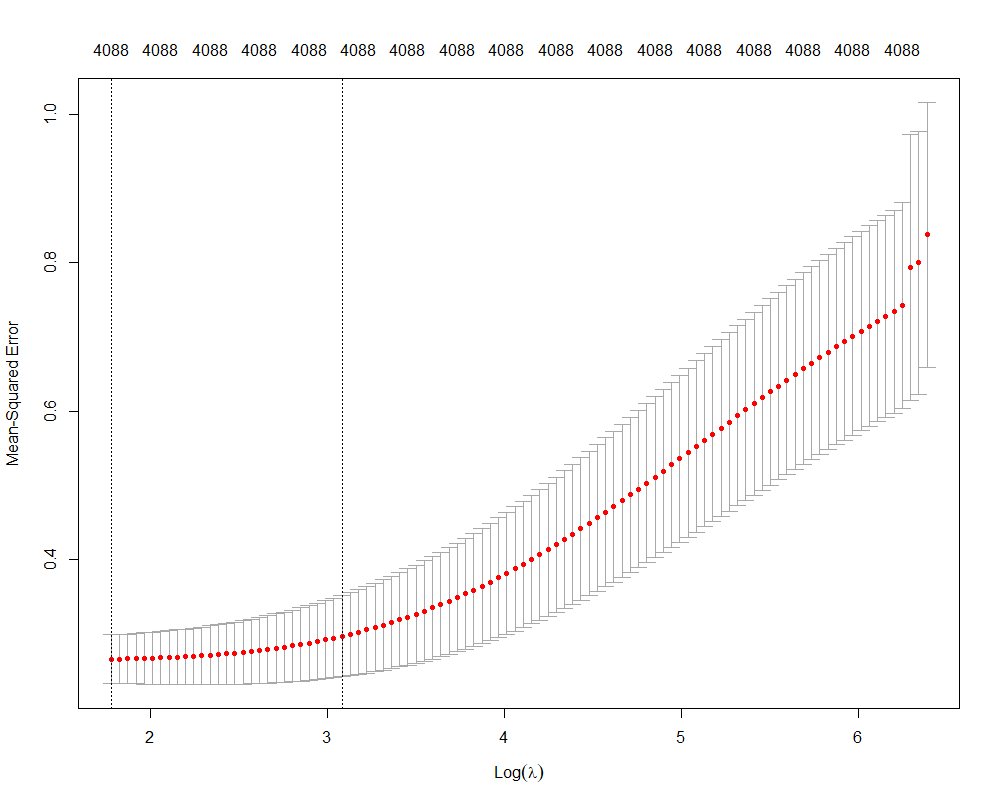
\includegraphics[width=0.45\textwidth]{MS1.png}}
\subfloat[]{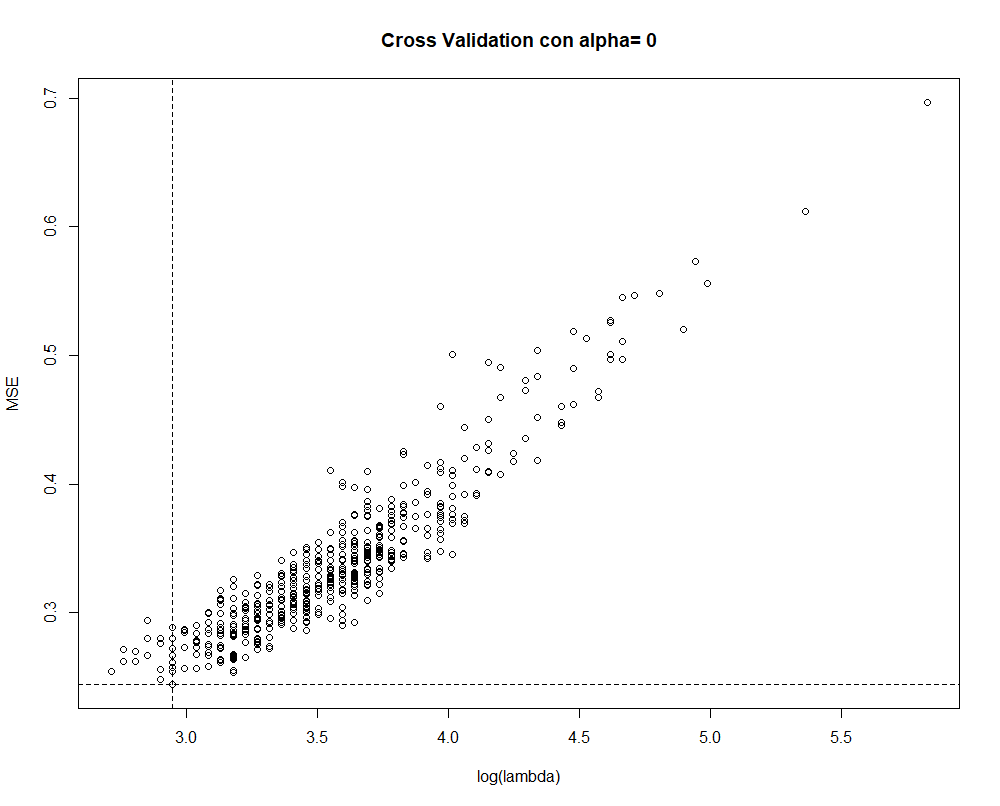
\includegraphics[width=0.45\textwidth]{MSCV1.png}} \hfill \hfill
\subfloat[]{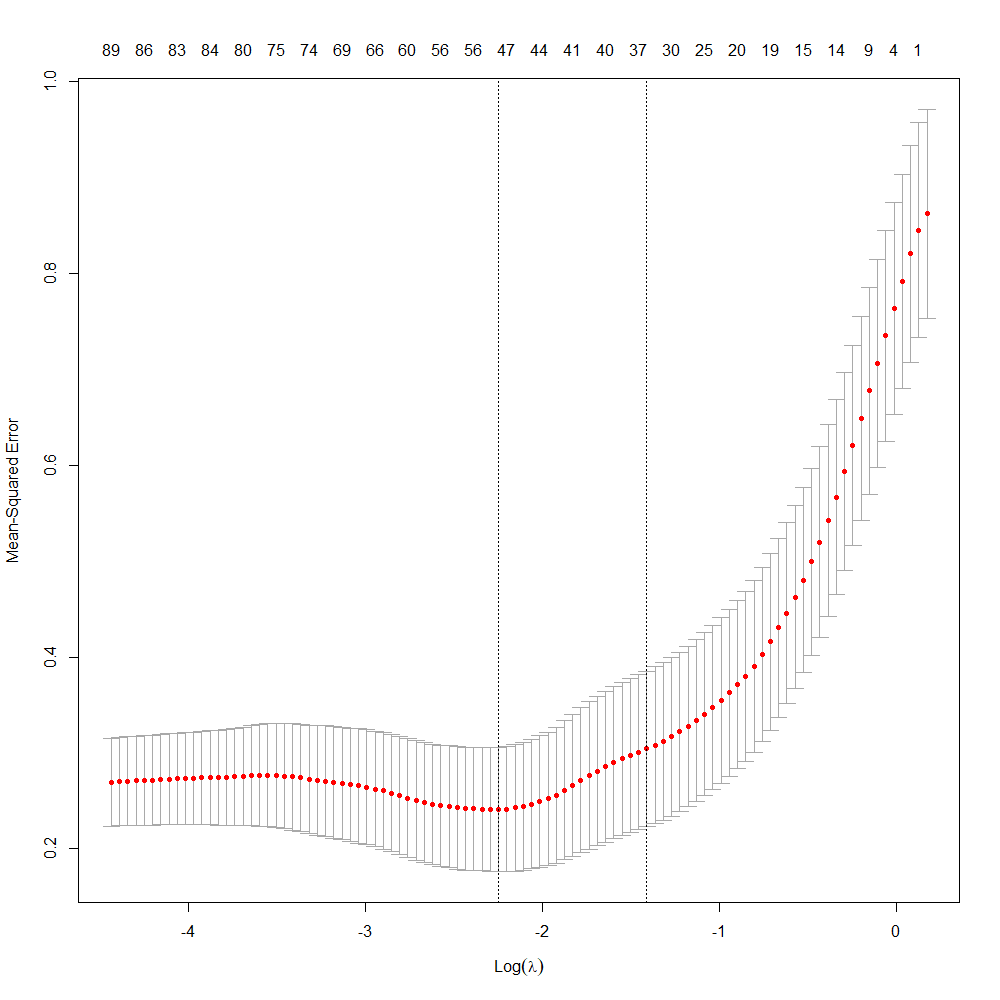
\includegraphics[width=0.45\textwidth]{MS2.png}}
\subfloat[]{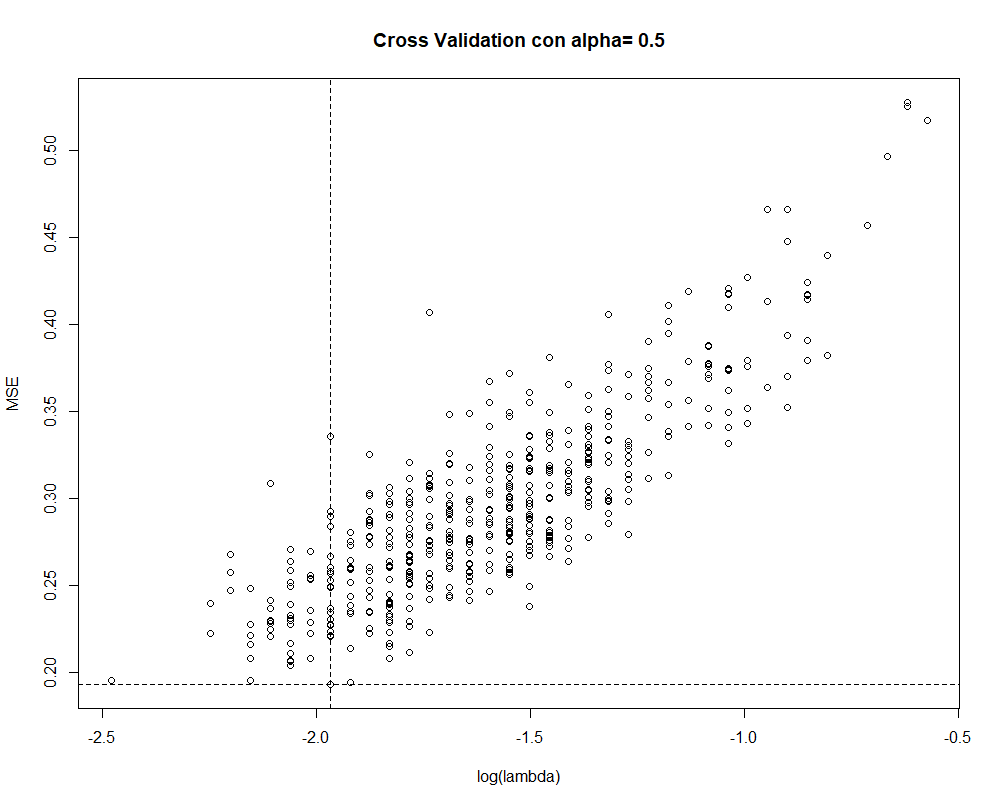
\includegraphics[width=0.45\textwidth]{MSCV2.png}} \hfill
\subfloat[]{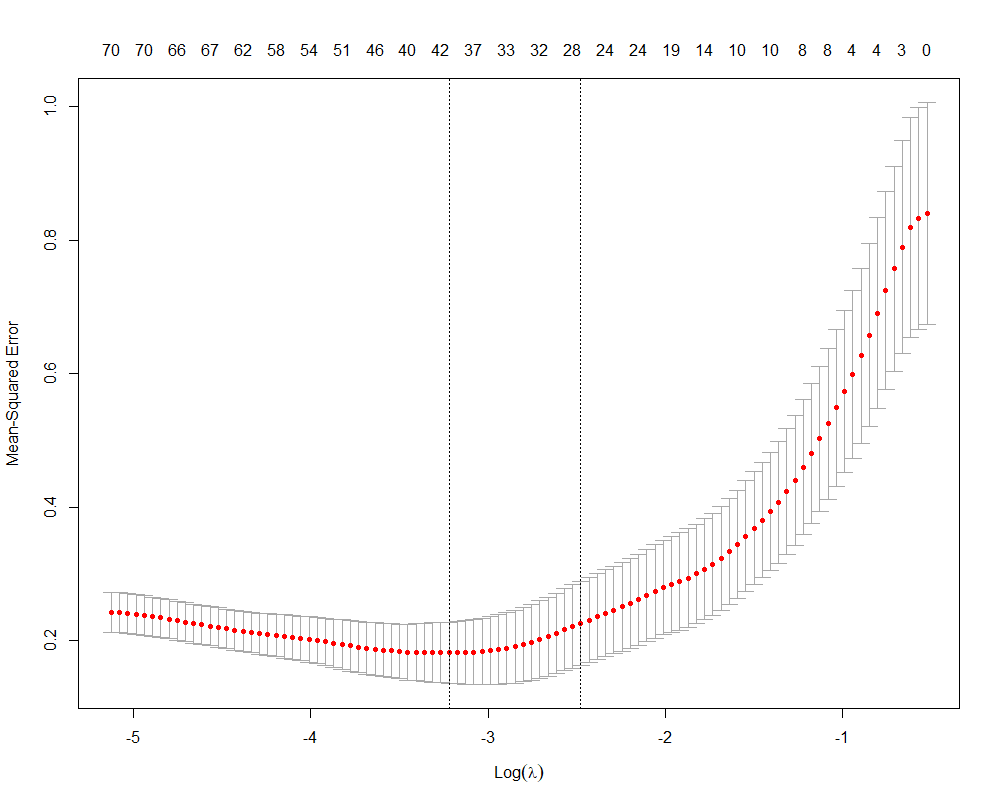
\includegraphics[width=0.45\textwidth]{MS3.png}}
\subfloat[]{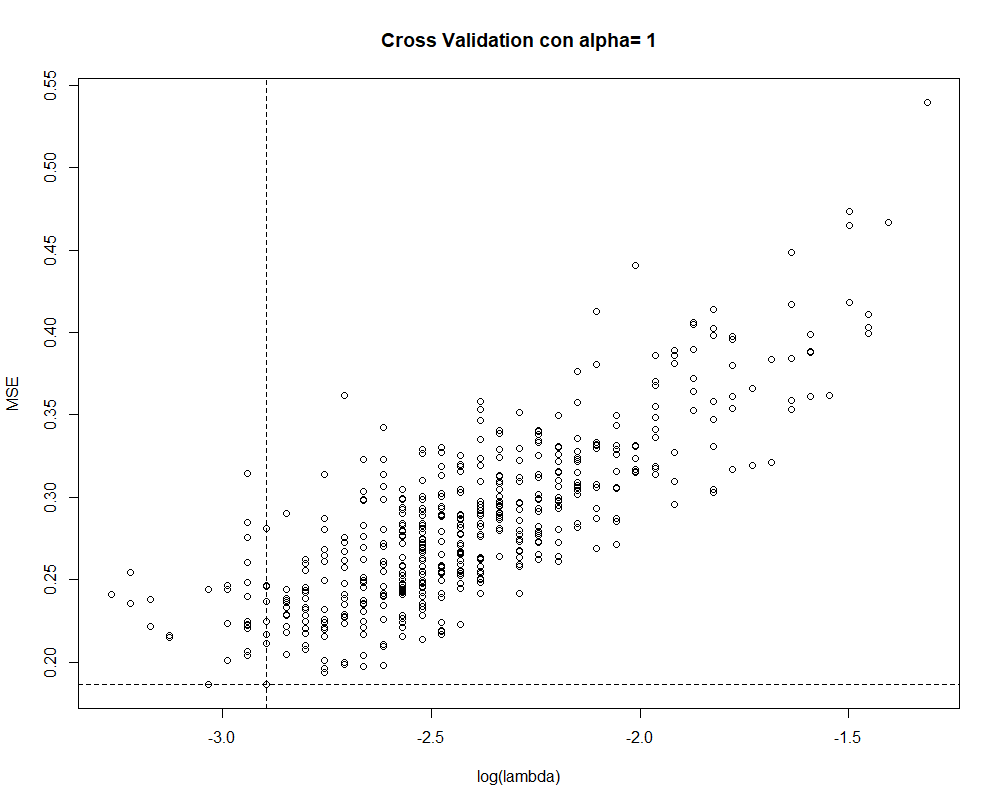
\includegraphics[width=0.45\textwidth]{MSCV3.png}} \hfill
    \caption{Perfiles de errores por Cross validataion para: (a) Ridge con 1 repetición; (b) Ridge con 500 repeticiones; (c) para Elastic Net con 1 repetición, (d) para Elastic Net con 500 repeticiones, (e) para Lasso con 1 repetición; (f) para Lasso con 500 repeticiones.}\label{fig:MS}
\end{figure}
\printbibliography
\end{document}
